\begin{activity}{Collisional Thermal Evolution}

\section*{Purpose}
The warm-up asked you to predict how heat flow evolves over the life cycle of an accretionary wedge and an orogen. This activity works through the orogen case using a real published thermal model: a thickened, initially hot crust relaxing toward a \emph{cooler} equilibrium, what that means for the thermal history of an individual rock parcel, and what real evidence exists for how long this relaxation actually takes.

\section*{Learning Outcomes}
By the end of this activity, you should be able to:
\begin{itemize}
  \item Predict how a perturbed (non-equilibrium) geotherm relaxes toward a lower-heat-flow equilibrium state, and identify which depths change fastest and slowest.
  \item Construct a qualitative pressure-temperature-time (P-T-t) path for a rock parcel undergoing decompression and cooling.
  \item Interpret real proxy data for the timescale of post-collisional thermal relaxation, and connect it to the steady-state assumption used elsewhere in this course.
\end{itemize}

\section*{Background: Fischer et al.'s Thermal Model}

Fischer et al.\ model collisional thermal relaxation as a crust cooling from a hot initial state to a cooler final one:
\begin{quote}
\small ``\ldots cool from a geotherm parameterized by initial surface heat flow ($q_0$) and crustal heat production ($A$) to an infinite time geotherm with lower heat flow ($q_f$) but the same $A$ value\ldots Initial thermal lithospheric thicknesses are 60--90~km and final thicknesses are 190--230~km\ldots Conductivity in all cases is 2.6~W\,m$^{-1}\,^\circ$C$^{-1}$, and mantle potential temperature is 1{,}300~$^\circ$C with an adiabatic gradient of 0.3~$^\circ$C\,km$^{-1}$.''
\end{quote}
This activity uses her $q_0=70$~mW/m$^2$ and $q_f=45$~mW/m$^2$ (the middle of her three $q_f$ cases), $A=0.7\ \mu$W/m$^3$ (held fixed, per her model), and a radiogenic layer 45~km thick -- a value not stated in her caption, chosen here because it reproduces her stated lithospheric thickness ranges almost exactly (71~km initial, 210~km final) when both states are treated as steady-state geotherms using the same method as your Week 8 activities.

\textbf{A caveat worth being explicit about:} holding $A$ fixed is a simplification. Part of why $q_f$ ends up lower than $q_0$ in real orogens is erosion -- stripping away radiogenic upper crust reduces the heat production actually available, not just the temperature. Fischer's model doesn't separate that from pure thermal relaxation; it just prescribes a lower $q_f$ as the net outcome. Keep both mechanisms in mind, even though the model itself only shows you one.

\begin{figure}[h]
    \centering
    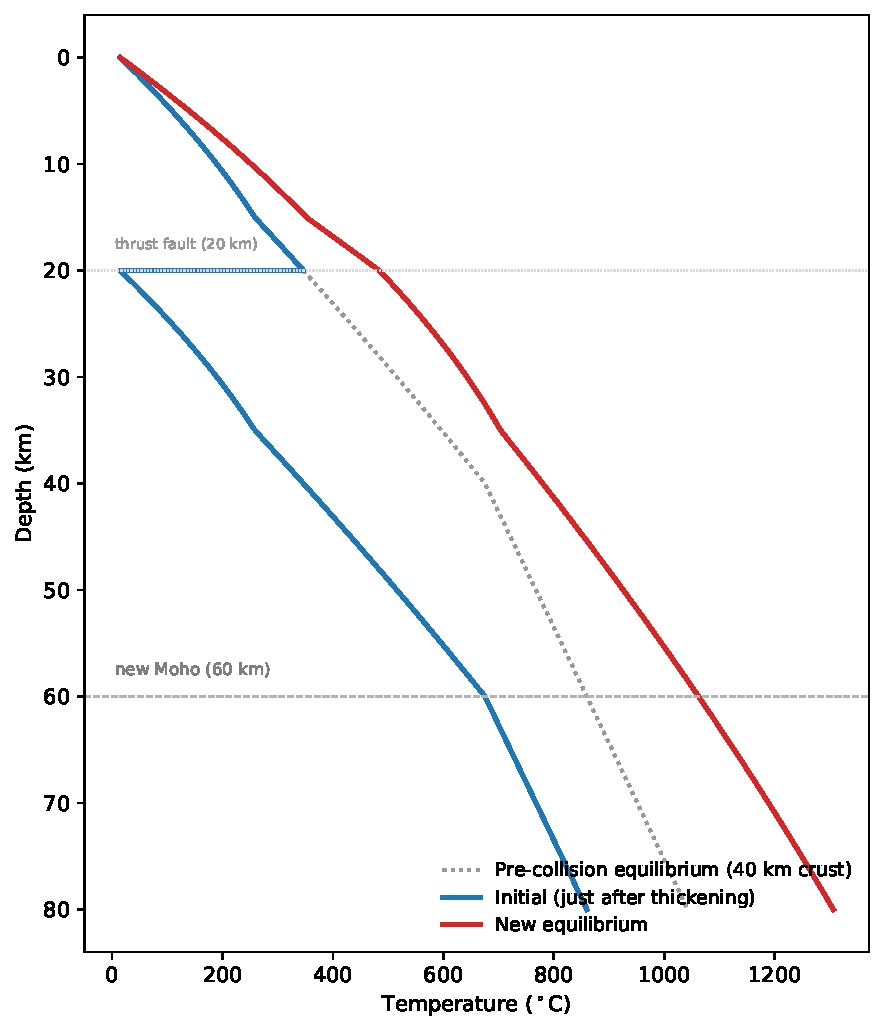
\includegraphics[width=0.6\textwidth]{figures/collisional_geotherms.pdf}
    \caption{Initial (red, $q_0=70$~mW/m$^2$) and final (blue, $q_f=45$~mW/m$^2$) steady-state geotherms, both with $A=0.7\ \mu$W/m$^3$ over a 45~km radiogenic layer, following Fischer et al.'s parameterization.}
    \label{fig:collisional}
\end{figure}

\section*{Tasks}
\begin{questions}

\question{Predicting the Relaxation}

\begin{enumerate}[label=(\alph*)]
  \item Two mechanisms could both make $q_f$ lower than $q_0$: the crust losing its initial excess heat by conduction, and erosion removing radiogenic material from the upper crust. Fischer's model only represents one of these explicitly (holding $A$ fixed) -- which one, and what would the other actually change in the equations if you tried to include it?
  \answerbox[2.5cm]

  \item On Figure~\ref{fig:collisional}, sketch how you'd expect the temperature at 30~km and at 100~km to evolve between the initial (red) and final (blue) curves. Which of your two depths do you expect to change faster, and why?
  \answerbox[2.5cm]

  \item What would you need to know to say \emph{how long} this relaxation actually takes, in years? (You don't need to compute it -- just state what's missing.)
  \answerbox[2cm]
\end{enumerate}

\question{A P-T-t Path}

Consider a rock parcel at 35~km depth in the initial (hot, $q_0$) state, which is then exhumed by erosion at a roughly constant rate, reaching 15~km depth by the time the column has relaxed most of the way to the final ($q_f$) state.

\begin{enumerate}[label=(\alph*)]
  \item Using your answer to Question 1, does this parcel's temperature rise, fall, or do both over this interval? (Careful: it is losing overburden \emph{and} sitting in a column that is itself cooling -- do both effects push temperature the same direction?)
  \answerbox[2.5cm]

  \item Sketch this parcel's path on a plot of pressure (proportional to depth) vs.\ temperature.
  \answerbox[3cm]

  \item This captures only the decompression-and-cooling half of the full path a real orogenic rock experiences -- metamorphic petrology typically teaches a full \emph{clockwise loop}, with an earlier burial-and-heating (prograde) stage this simplified two-endpoint model doesn't include. Why might a model that starts already-thickened and already-hot be a reasonable simplification for studying the relaxation timescale specifically, even though it skips how the rock got there?
  \answerbox[2.5cm]
\end{enumerate}

\question{Real Evidence: Root Decay Through Time}

Fischer et al.\ compiled $R$ -- as best can be determined without the original paper's full methods, the ratio of surface relief (topographic height relative to the surrounding plain, not elevation above sea level) to crustal root thickness -- for orogens of many different ages. For a fixed root, $R$ tracks the buoyancy that root is actually providing per unit thickness -- so as a root cools and densifies toward normal mantle density, the same root thickness supports less relief, and $R$ falls, even before the root itself has shrunk.

\begin{figure}[h]
    \centering
    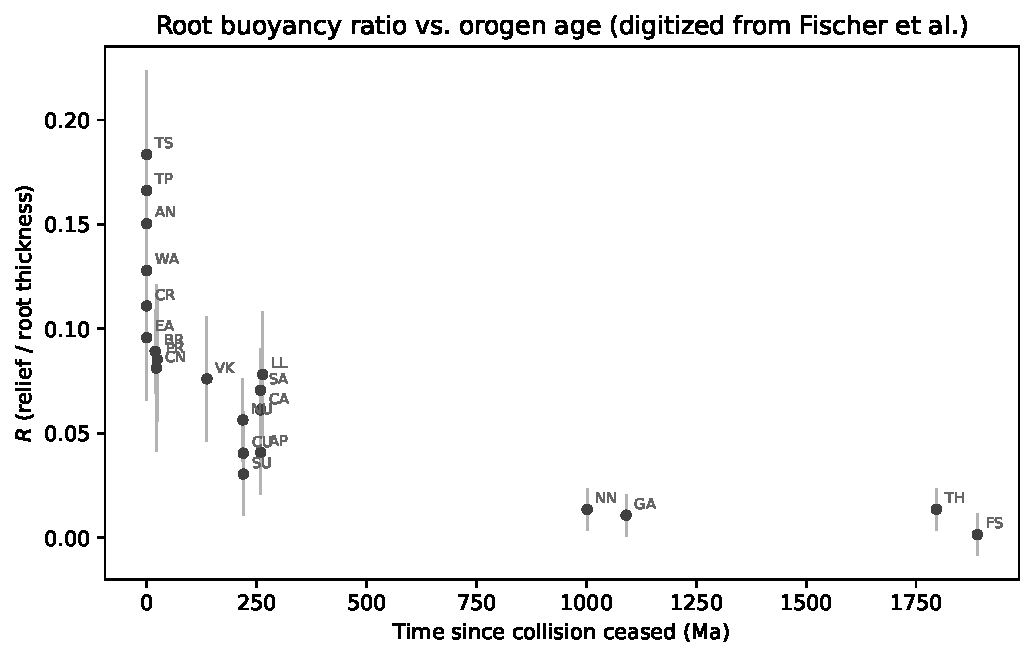
\includegraphics[width=0.85\textwidth]{figures/R_vs_age.pdf}
    \caption{$R$ vs.\ time since collision ceased, digitized from Fischer et al., all ages shown. Error bars are per-point estimated uncertainties (one-sided estimates, applied symmetrically).}
    \label{fig:fischerR}
\end{figure}

\begin{figure}[h]
    \centering
    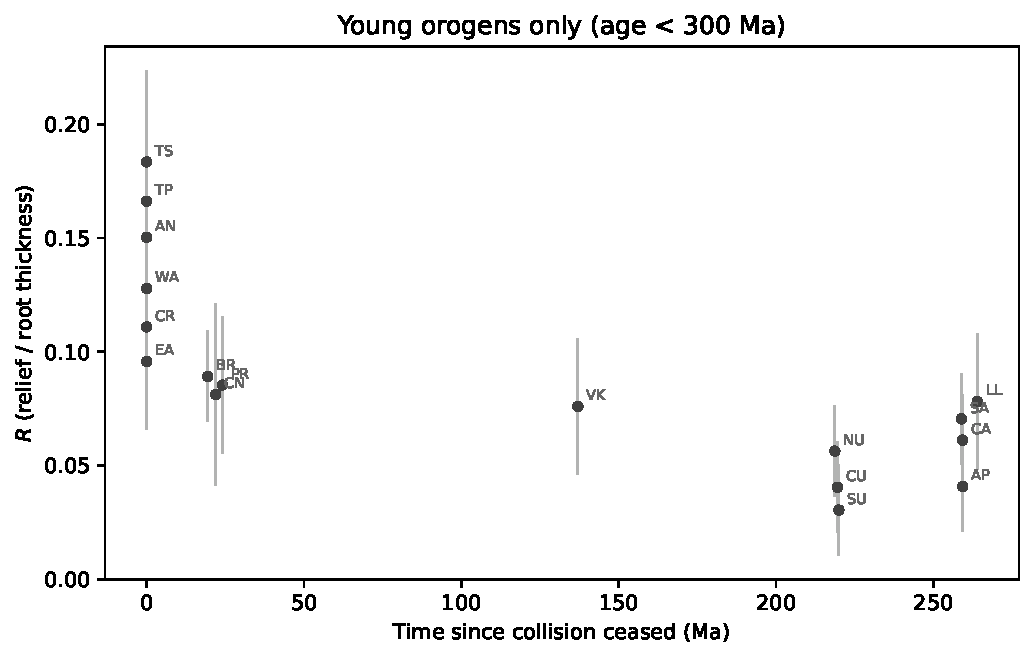
\includegraphics[width=0.85\textwidth]{figures/R_vs_age_young.pdf}
    \caption{Same data, young orogens only (age $<300$~Ma).}
    \label{fig:fischerR_young}
\end{figure}

\begin{enumerate}[label=(\alph*)]
  \item Does $R$ decay smoothly with age, or does it flatten out at some point the way plate-cooled oceanic lithosphere does?
  \answerbox[2cm]

  \item Week 8's problem set computes thermal isostasy \emph{assuming} steady state. Based on these figures, roughly how old does an orogen need to be before that assumption is reasonable?
  \answerbox[2.5cm]

  \item Both this activity's model and the oceanic cooling activity describe a column relaxing away from an initial thermal anomaly. Given that both relax via the same kind of physics, would you expect $R(t)$ to follow the same functional form as oceanic $q(t)$, oceanic $s(t)$, neither, or is there not enough information in this figure alone to tell?
  \answerbox[2.5cm]
\end{enumerate}

\question{Estimating Heat Flow from $R$ -- [Placeholder]}

\textit{This section is still in development. Fischer's own $q_0=70$~mW/m$^2$ and $q_f=45$~mW/m$^2$ are natural calibration anchors for the youngest and oldest ends of the $R$ curve -- the calibration points earlier identified as missing may now be available. Plan: use these anchors to convert $R(t)$ into an estimated heat-flow-through-time curve for collisional orogens, the collisional counterpart to the oceanic figure from the last activity.}

\end{questions}

\section*{Key Ideas}

\textbf{A thickened column's surface heat flow can fall as it relaxes, not just rise.} Which direction depends on the mechanism: burying radiogenic crust deeper (trapping its heat) raises the eventual equilibrium; losing an initial excess of heat -- whether from syn-collisional heating, magmatism, or simply not yet having conducted away -- lowers it. Real orogens likely involve both, plus erosion actively removing radiogenic mass, which Fischer's fixed-$A$ model doesn't separately represent.

\textbf{The same relaxation shows up as two different observables, on two different timescales of confidence.} Temperature evolution is what the physics predicts directly; $R$ (relief per unit root thickness) is what can actually be measured, for real orogens, over geological time. Neither alone tells the whole story.

\textbf{A P-T-t path is a rock's biography, not a snapshot.} Everything else in this course has asked "what does the geotherm look like right now" -- a P-T-t path asks what a single parcel experienced on its way to wherever it ended up. This activity only shows half of it (decompression and cooling); the full clockwise loop taught in metamorphic petrology also includes how the rock got buried and hot in the first place.

\end{activity}
